% Auto-generated from committed gate JSONs by generate_figures.py. Do not edit by hand.

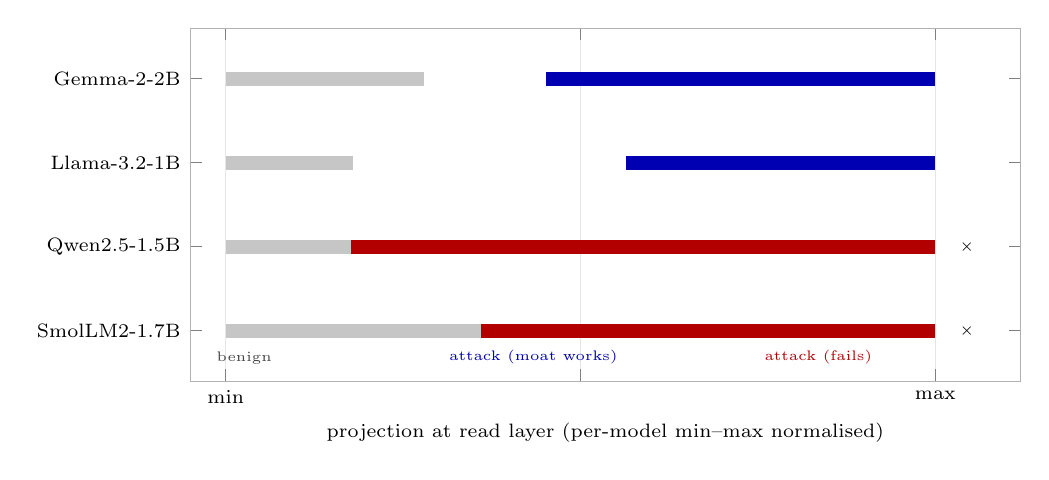
\begin{tikzpicture}
\begin{axis}[
  width=\columnwidth, height=0.5\columnwidth,
  xmin=-0.05, xmax=1.12, ymin=0.4, ymax=4.6,
  xlabel={projection at read layer (per-model min--max normalised)},
  xtick={0,0.5,1}, xticklabels={min,,max},
  ytick={4,3,2,1}, yticklabels={Gemma-2-2B,Llama-3.2-1B,Qwen2.5-1.5B,SmolLM2-1.7B},
  label style={font=\scriptsize}, tick label style={font=\scriptsize},
  axis line style={gray!60}, xmajorgrids, grid style={gray!20},
]
\addplot[draw=none] coordinates {(0,1)};
\draw[line width=5pt, gray!45] (axis cs:0.000,4) -- (axis cs:0.280,4);
\draw[line width=5pt, blue!70!black] (axis cs:0.452,4) -- (axis cs:1.000,4);
\node[font=\tiny, anchor=west] at (axis cs:1.02,4) {\checkmark};
\draw[line width=5pt, gray!45] (axis cs:0.000,3) -- (axis cs:0.179,3);
\draw[line width=5pt, blue!70!black] (axis cs:0.564,3) -- (axis cs:1.000,3);
\node[font=\tiny, anchor=west] at (axis cs:1.02,3) {\checkmark};
\draw[line width=5pt, gray!45] (axis cs:0.000,2) -- (axis cs:0.405,2);
\draw[line width=5pt, red!70!black] (axis cs:0.176,2) -- (axis cs:1.000,2);
\node[font=\tiny, anchor=west] at (axis cs:1.02,2) {$\times$};
\draw[line width=5pt, gray!45] (axis cs:0.000,1) -- (axis cs:0.447,1);
\draw[line width=5pt, red!70!black] (axis cs:0.360,1) -- (axis cs:1.000,1);
\node[font=\tiny, anchor=west] at (axis cs:1.02,1) {$\times$};
\node[font=\tiny, gray!55!black, anchor=south west] at (rel axis cs:0.02,0.02) {benign};
\node[font=\tiny, blue!70!black, anchor=south west] at (rel axis cs:0.30,0.02) {attack (moat works)};
\node[font=\tiny, red!70!black, anchor=south west] at (rel axis cs:0.68,0.02) {attack (fails)};
\end{axis}
\end{tikzpicture}
